\documentclass{article}
\usepackage{color}
\usepackage{placeins}
\usepackage{listings}
\usepackage{graphicx}
\usepackage{xcolor}
\usepackage{amsmath}
\usepackage{subcaption}
\usepackage{cleveref}
\usepackage{geometry}[margins=1in]
\setlength{\parskip}{4pt plus 2pt}
\setlength{\parindent}{0pt}
%\pagecolor[rgb]{0,0,0} %black
%\color[rgb]{1,1,1} %grey
\lstset{language=C++,
keywordstyle=\color{blue},
stringstyle=\color{red},
commentstyle=\color{green},
morecomment=[l][\color{magenta}]{\#},
breaklines=true,
breakatwhitespace=true,
numbers=left
}
\title{Assignment \#4}
\author{Asbjørn Bonefeld Preuss,\\ Daniel Lomholt Christensen,\\ Elie Cueto}
\date{March 2024}

\begin{document}
\maketitle
\section{Task \#1}
In order to parallelise the code, we first profiled the sequential code. This result can be seen in appendix \ref{sec:Profiling}. The profiling showed that our initial effort should be concentrated around the propagator function, and then next address the fourier transformation, and finally the inverse fourier transformation.

The propagator function was parallelised by first beginning a parallel block on line 178, as soon as all the important declarations and initialisations are done. This block ends just before the function prints out the debugging information and ends the time taking, at line 278. 

Inside the parallel block, all for loops are given an omp for directive, thus spreading the loop iterations over the threads. Omp single directives are used when only one thread must execute the code. This is all that was used to parallelise the propagator function.

Next, the fast fourier transformation(lines 104-129) was parallelised. Since the fft is a recursive function, the most important part to parallelise is the calling of the function itself. We do not want to parallelise the for loops, because each time the function is called a new, the threads must be spun up anew, as they cannot be used for calling the function again.

The fft calls inside the fft function are therefore just given to a thread, and then the computer is asked to wait until the tasks finish.

Finally the inverse fast fourier transform(lines 132-152) is parallelised. The ifft is run in parallel, with the two loops getting the omp for directive, and the fft call given on only a single thread. The second loop is split, into a vectorisable part and non-vectorisable part, and given the appropriate directives to compile it correctly.

The overall strategy is therefore to parallelise what can be parallelised, if there is any gain to be made from the parallelisation.

We tested that the checksum is the same, 23.2912755963295 for the vectorised, and 23.2912755963295 for the sequential code, run with $n_{freq}=2^{16}$. 

\section{Task \#2}
\subsection{Strong scaling}


\appendix
\newpage
\section{Profiling}
\label{sec:Profiling}
\begin{figure}[h]
    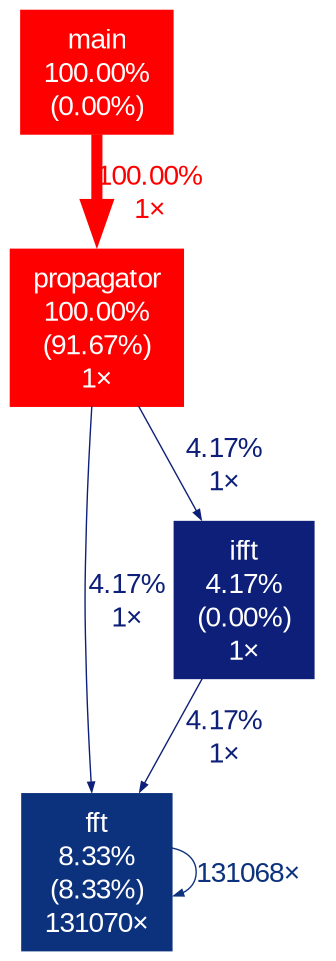
\includegraphics[height=0.6\textheight]{figures/gprof_seq.png}
    \centering
    \caption*{Profiling of the sequential program.}
\end{figure}
\FloatBarrier
\section{Source Code}
\label{sec:source}
\lstinputlisting[language=c++]{../Code/seismogram_omp.cpp}

\end{document}
